\documentclass[tikz,border=2pt]{standalone}
\usepackage{amsmath,amssymb}
\usepackage{tikz}

\begin{document}
% Zero-inventory ordering: an order is placed only when the starting stock is zero and it
% covers whole consecutive periods (four-period example: orders 61, 116, 0, 67 cover period 1,
% periods 2-3 and period 4).
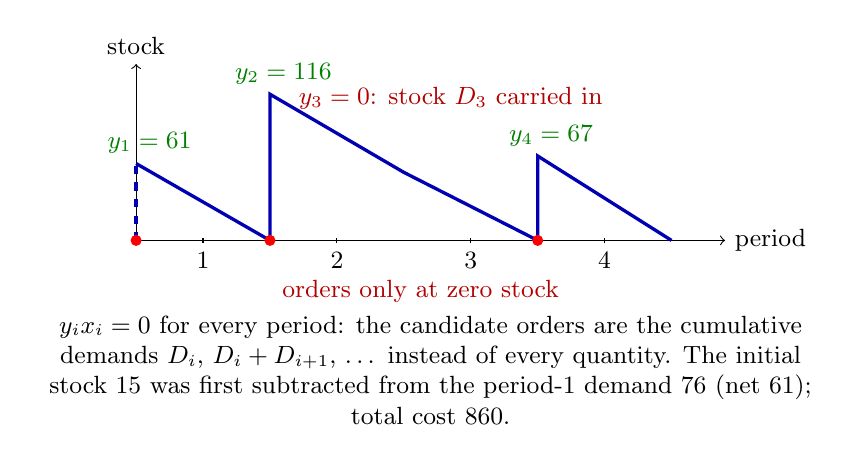
\begin{tikzpicture}[every node/.style={font=\small}, x=1.7cm, y=0.016cm]
	\draw[->] (0,0) -- (4.4,0) node[right] {period};
	\draw[->] (0,0) -- (0,140) node[above] {stock};
	\foreach \i in {1,2,3,4} {\draw ({\i-0.5},2) -- ({\i-0.5},-2) node[below] {$\i$};}
	\draw[blue!70!black, very thick] (0,61) -- (1,0) -- (1,116) -- (2,54) -- (3,0) -- (3,67) -- (4,0);
	\draw[blue!70!black, very thick, dashed] (0,0) -- (0,61);
	\foreach \x/\y/\l in {0/61/{$y_1=61$}, 1/116/{$y_2=116$}, 3/67/{$y_4=67$}} {\node[green!50!black, anchor=south] at ({\x+0.1},\y) {\l};}
	\node[red!70!black, anchor=south] at (2.35,96) {$y_3=0$: stock $D_3$ carried in};
	\fill[red] (1,0) circle (2pt); \fill[red] (3,0) circle (2pt); \fill[red] (0,0) circle (2pt);
	\node[red!70!black, anchor=north west] at (1.02,-24) {orders only at zero stock};
	\node[anchor=north, align=flush center, text width=10cm] at (2.2,-52) {$y_ix_i=0$ for every period: the candidate orders are the cumulative demands $D_i$, $D_i+D_{i+1}$, \dots\ instead of every quantity. The initial stock $15$ was first subtracted from the period-1 demand $76$ (net $61$); total cost $860$.};
\end{tikzpicture}
\end{document}
